% This file was created by tikzplotlib v0.9.8.
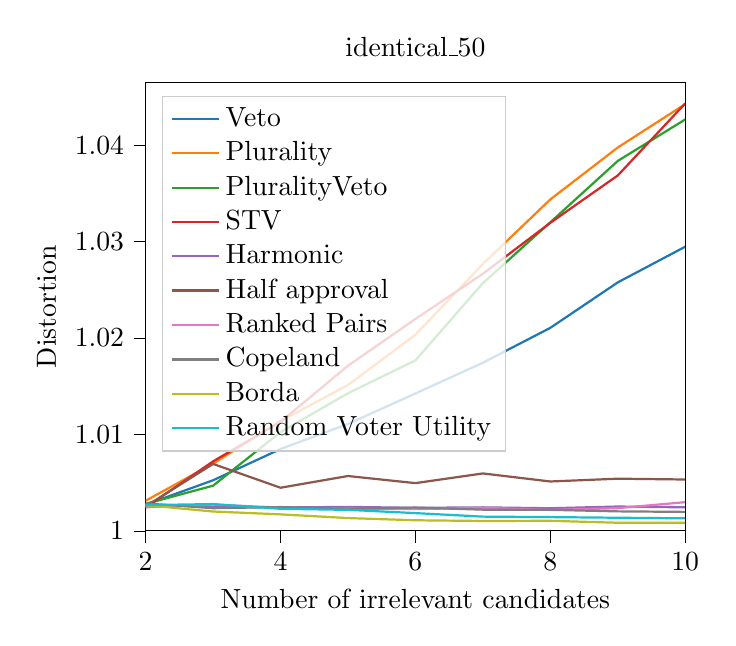
\begin{tikzpicture}

\definecolor{color0}{rgb}{0.12156862745098,0.466666666666667,0.705882352941177}
\definecolor{color1}{rgb}{1,0.498039215686275,0.0549019607843137}
\definecolor{color2}{rgb}{0.172549019607843,0.627450980392157,0.172549019607843}
\definecolor{color3}{rgb}{0.83921568627451,0.152941176470588,0.156862745098039}
\definecolor{color4}{rgb}{0.580392156862745,0.403921568627451,0.741176470588235}
\definecolor{color5}{rgb}{0.549019607843137,0.337254901960784,0.294117647058824}
\definecolor{color6}{rgb}{0.890196078431372,0.466666666666667,0.76078431372549}
\definecolor{color7}{rgb}{0.737254901960784,0.741176470588235,0.133333333333333}
\definecolor{color8}{rgb}{0.0901960784313725,0.745098039215686,0.811764705882353}

\begin{axis}[
legend cell align={left},
legend style={
  fill opacity=0.8,
  draw opacity=1,
  text opacity=1,
  at={(0.03,0.97)},
  anchor=north west,
  draw=white!80!black
},
tick align=outside,
tick pos=left,
title={identical\_50},
x grid style={white!69.0196078431373!black},
xlabel={Number of irrelevant candidates},
xmin=2, xmax=10,
xtick style={color=black},
y grid style={white!69.0196078431373!black},
ylabel={Distortion},
ymin=1, ymax=1.04650518024628,
ytick style={color=black}
]
\addplot [thick, color0]
table {%
2 1.00271427237274
3 1.00524123231911
4 1.00848457879831
5 1.01108119308146
6 1.01424444809109
7 1.01743276052889
8 1.02105271493402
9 1.0257693899965
10 1.02947001065148
};
\addlegendentry{Veto}
\addplot [thick, color1]
table {%
2 1.00311531009361
3 1.00696128499614
4 1.0113933424849
5 1.01512488979406
6 1.02033788507693
7 1.02767800928085
8 1.0343767876066
9 1.03976089463585
10 1.0442641289507
};
\addlegendentry{Plurality}
\addplot [thick, color2]
table {%
2 1.00279236523174
3 1.00468117130304
4 1.01023519319084
5 1.01426847135364
6 1.01768038797139
7 1.02568789901584
8 1.03200207439082
9 1.0383685597303
10 1.04267309858196
};
\addlegendentry{PluralityVeto}
\addplot [thick, color3]
table {%
2 1.00241503405246
3 1.00720106059529
4 1.01129890490656
5 1.01711908599807
6 1.02197373325358
7 1.02666544472778
8 1.0319499620756
9 1.03686170135362
10 1.04433046029005
};
\addlegendentry{STV}
\addplot [thick, color4]
table {%
2 1.00270848473191
3 1.00249552437382
4 1.00242027016075
5 1.00248010405969
6 1.0023836297123
7 1.00243327314902
8 1.00233923848623
9 1.00251980586159
10 1.0024331322753
};
\addlegendentry{Harmonic}
\addplot [thick, color5]
table {%
2 1.00253564712421
3 1.00693734345593
4 1.00446824274269
5 1.00568343224343
6 1.00494693996881
7 1.00595064371505
8 1.00511665616067
9 1.00540619826112
10 1.00532208678968
};
\addlegendentry{Half approval}
\addplot [thick, color6]
table {%
2 1.00243953738918
3 1.00272088275809
4 1.00240557875019
5 1.00231178493446
6 1.00224980397267
7 1.00238090431109
8 1.00216478406337
9 1.00234917922627
10 1.00297270424131
};
\addlegendentry{Ranked Pairs}
\addplot [thick, white!49.8039215686275!black]
table {%
2 1.00284149821338
3 1.00234520166453
4 1.00246326351094
5 1.00228751356492
6 1.00241109413204
7 1.00219479692843
8 1.00217460941214
9 1.00201687508655
10 1.00196217566728
};
\addlegendentry{Copeland}
\addplot [thick, color7]
table {%
2 1.00265714925035
3 1.00200173968234
4 1.0017064458292
5 1.00132121286588
6 1.00109272316431
7 1.00101978580608
8 1.00103746137775
9 1.00083606116548
10 1.00084531076852
};
\addlegendentry{Borda}
\addplot [thick, color8]
table {%
2 1.00266808672984
3 1.00277149533468
4 1.00228206533661
5 1.00217387989642
6 1.0018357480712
7 1.00147113768221
8 1.00142131292745
9 1.00135487819111
10 1.00129631810525
};
\addlegendentry{Random Voter Utility}
\end{axis}

\end{tikzpicture}
